\customHeader{0}{Practical Implications and Future Work}
\label{08_practical_implications}


In this \headerName{}, we discuss the real-world impact of our research, detailing its application, updates, and the effects it will have on the work of the \gls{vsi} experts.

\customHeader{1}{Overview}
\label{08_overview}


Upon determining the optimal hyperparameters for the most effective classifiers (as seen in Table \ref{tab:07_best_classifiers}), the \gls{pesv} team plans to integrate our findings into their data collection pipeline as a component of the \gls{tiersesv} initiative.

For the \gls{tiersesv} project, we have developed two key services:
\begin{itemize}
\item A service for inference.
\item A service for training.
\end{itemize}



\customHeader{1}{Inference Service}
\label{08_inference_service}


\begin{figure}[h]
    \centering
    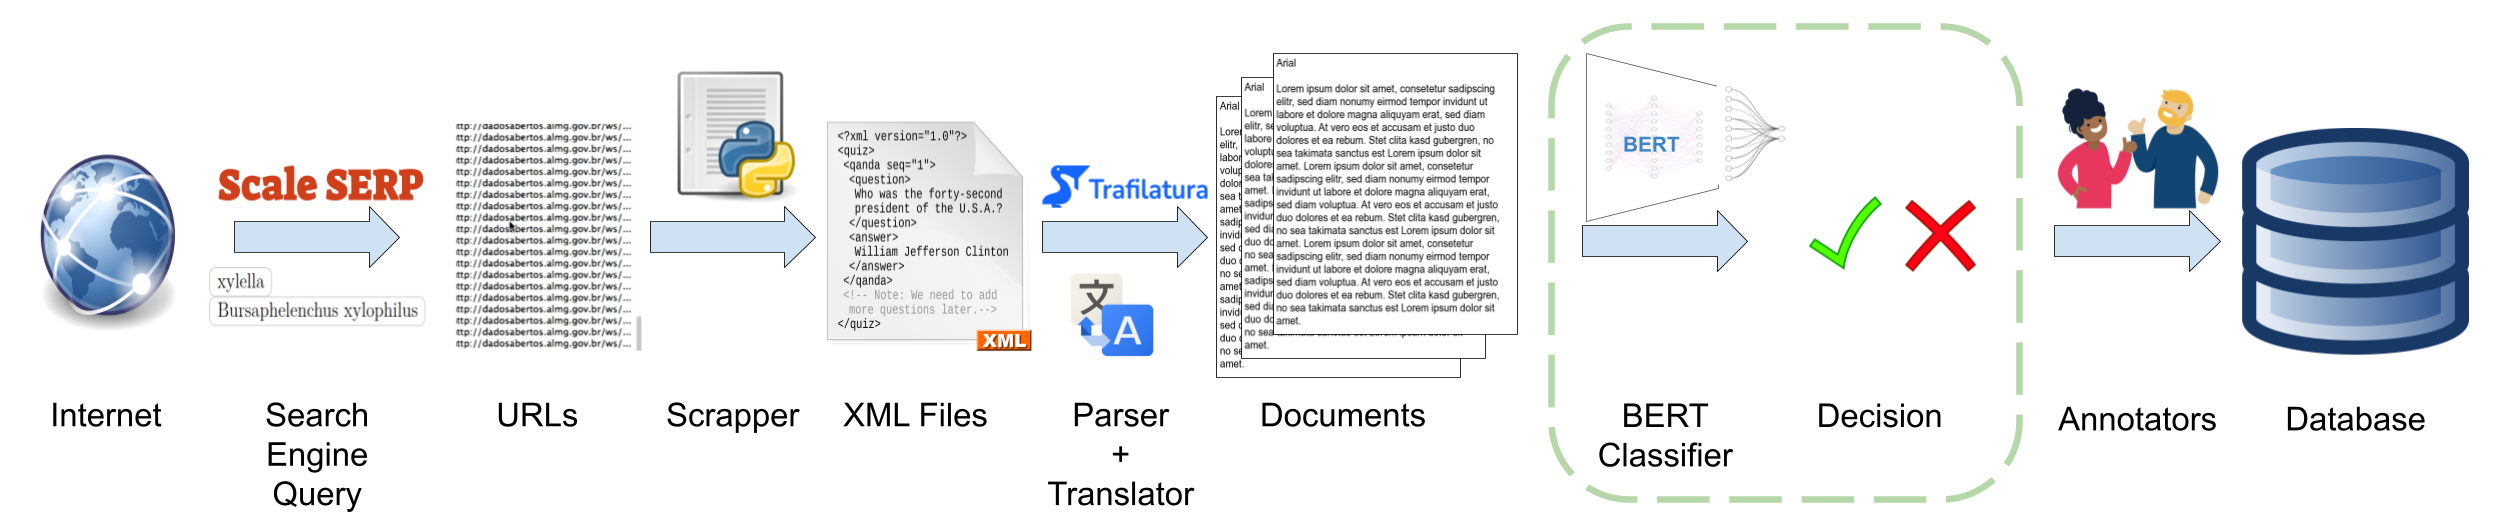
\includegraphics[width=\textwidth]{Figures/08/08_vsi_dataset_collection_with_classifier.png}
    \caption{Our classifiers added to the \VSI{} Data Collection Pipeline}
    \label{fig:08_vsi_data_collection_pipeline_with_classifier}
\end{figure}

Our Document Classification system will be integrated into the \gls{vsi} data collection pipeline, as depicted in Figure \ref{fig:08_vsi_data_collection_pipeline_with_classifier}. This system is composed of two primary components:
\begin{enumerate}
\item Heuristic methods
\item Neural-based \textclassification{}
\end{enumerate}

The heuristic component is designed to eliminate entries that lack substantial content. For those documents that do contain content, the \textclassification{} component of the system applies our trained models.
The results produced by this filter will be fed into the \gls{vsi} database. Overall, we anticipate that this addition will significantly reduce the manual effort required by the \gls{vsi} experts.

The implementation of this filter will utilize the Python package developed during this thesis.


\begin{enumerate}

    \item First, the results from web scraping, as an XML/TEI file, are processed using our tool to extract the \trafilaturaTitle{}, the \trafilaturaAbstract{}, the \trafilaturaFulltext{}, and the \translationTitle{}.
    
    \item Subsequently, any noise such as HTML tags, URLs, website names, and the like are filtered out from the text for each \contentType{}.

    \item The heuristic module then employs the tools we developed for preprocessing. By using functions that identify error messages and scraping issues, one can eliminate document that lack substantial content.

    \item  Then, for each \contentType{}, the cleaned text is given as input for the \textclassification{} model.

    \item Finally, the output of the filter for a particular document consists of
    \begin{itemize}
        \item A boolean flag indicating whether the document was kept.
        \item The cleaned text
        \item The prediction: Relevant VS Irrelevant
        \item The label probabilities
    \end{itemize}


\end{enumerate}

Given our observations on addressing error messages and managing scraping errors (as discussed in \headerName{}s \ref{vsi_deleting_error_messages} and \ref{05_vsi_handling_scrapping_errors}), we anticipate that the heuristic model will exclude between 20\% to 30\% of unique documents, depending on the \contentType{}.

This filtering system will be applied to the documents scraped weekly by the \gls{pesv} Platform. 
For user convenience, it will be encapsulated within a \texttt{REST} API, hosted on the \MAIAGE{} servers, and integrated into the \href{https://bibliome.github.io/alvisnlp/)}{\emph{AlvisNLP-ML}}\footnote{\url{https://bibliome.github.io/alvisnlp/}} toolkit of the \bibliome{} group \myparencite{alvisnlp}. 
Lastly, when publishing selected documents in the official bulletin of the \gls{pesv} Platform, they will be arranged in order of decreasing relevance.



\customHeader{1}{Training Service}
\label{08_training_service}

As the \gls{vsi} Database expands with new entries, there will be a need to update the models utilized for \textclassification{}. This responsibility falls on the training service, which implements the entire pipeline to train the best performing classifiers from Table \ref{tab:07_best_classifiers}.

The frequency and data selection for training will be at the discretion of the \gls{vsi} experts. They must determine whether training should occur weekly, bi-weekly, etc. Additionally, as their priorities and interests evolve, they might find it beneficial to limit the training data, perhaps only focusing on data from recent months.

The training service is designed to run on the \texttt{Lab-IA} cluster. All scripts related to this service can be found in our GitLab repository.



\customHeader{1}{Consequences for Plant Health Surveillance}
\label{08_consequences}


Until now, the \gls{vsi} experts at the \gls{pesv} Platform have been meticulously reviewing every scraped document. 
Integrating \textclassification{} into the annotation process will significantly reduce the burden on the \gls{vsi} experts, ultimately aiding in long-term Plant Health Surveillance.

By incorporating the Heuristics module, the \gls{vsi} experts can identify which queries and websites pose challenges for their scraping tools.

Given that the \gls{vsi} experts will review documents marked as Relevant by our system, we decided to calculate the positive ratio for the top classifiers on their respective test splits. Moreover, we aim for a reduced rate of false negatives, meaning the percentage of genuinely Relevant documents that our system mistakenly labels as Irrelevant (refer to Table \ref{tab:08_ratio_of_positives}). The rationale behind this is that overlooking an event that poses a risk to Plant Health (a positive) is more dangerous than mistakenly identifying a harmless event (a negative) as Relevant.


\begin{table}[ht]
\centering
\resizebox{\textwidth}{!}{
\begin{tabular}{|ccccc|}
\hline
  \contentType{}                                   & Model & Training Method & Positives/Total & FN/Total \\ \hline
  \trafilaturaTitle{} & \bertmultilingual{} & \petThousand{}  & 43.33\% & 2.0\%\\ \hline %0.43333333333333335 \\

 \trafilaturaAbstract{} & \bertxlmroberta{} & \petThousand{} & 40.16\% & 2.23\% \\  \hline %0.4016489988221437 \\
\trafilaturaFulltext{} & \bertmultilingual{} & \petThousand{} & 26.55\% & 1.66\%\\%0.29547471162378 \\ 
\trafilaturaFulltext{} & \bertxlmroberta{} & \balanced{} & 24.16\% &  2.89\%\\%0.24156305506216696 \\
\trafilaturaFulltext{} & \bertxlmroberta{} & \petThousand{} & 37.27\% & 1.20\% \\ %0.37267080745341613 \\
\hline
\translationTitle{} & \bertmultilingual{} & \petThousand{} & 34.62\% & 1.69\% \\ %0.34615384615384615 \\
\hline
\end{tabular}
}
\caption{Positives and FN ratios for the best classifiers}
\label{tab:08_ratio_of_positives}
\end{table}


The minimal False Negative rates indicate that our systems will overlook only around 2 out of every 100 Relevant (unique) documents, which we view as an impressive outcome. 
As mentioned in \headerName{} \ref{vsi_results_of_preprocessing}, the actual  proportions in the \gls{vsi} Dataset fluctuate between 12\% and 14\% positives. The closer our classifiers approach to this balance, the fewer documents the \gls{vsi} experts will need to review manually.

In the most favorable scenario, with a Positive ratio of $24\%$, the \gls{vsi} experts will encounter roughly $76\% \approx 3/4$ fewer documents than they currently do. Conversely, in the least favorable scenario, with a Positive ratio of $43\%$, they will see about $57\% \approx 1/2$ fewer documents.


\putInBox{
This demonstrates that integrating our system into their monitoring mission will significantly decrease the number of documents requiring manual review. This will allow the \gls{vsi} experts to either assess the same volume of documents more quickly, allocate the same time to evaluate a larger set of documents, or broaden their surveillance to additional pathogens. We consider this outcome to be satisfactory and a fitting conclusion to our work.
}


\clearpage


% Heuristics
% NLP

% noticing which websites are problematic for their tool

\iffalse


1. Dans le workflow de travail de la Plateforme ESV, il est déjà prévu un slot pour le filtrage automatique de documents.


    Search (Google) -> Extract (Proprietary) -> Extract (Trafilatura) -> Traduction titre (Google) [-> Filter (you)] -> Traduction fulltext (Google) -> Presentation (Proprietary, screenshot) -> Examination (Humans)


2. Le projet TIERS-ESV vise à étudier les apports possibles des technologies du NLP pour la veille épidémiologique. Participants: Bibliome, Migale, Plateforme ESV.


3. Le projet TIERS-ESV devra choisir un modèle pour l'étape de filtrage.

Critères:

    - performances: R/P/F1/F2 mais aussi balance entre Faux Négatifs (1/R) et Taux de Positifs ( (TP+FP)/N )

    - temps d'entraînement et d'inférence


3. Le projet TIERS-ESV fera de ce modèle un service:

    - entraînement et inférence automatisées
    
    - commandable à distance

    - fréquence: 1 semaine

    - décisions: fréquence d'entraînement, ensemble d'entraînement. Critères: temps d’entraînement, actualité deu filtrage par rapport à la perspective des agents. train with the last three months


4. Outils d'intégration

    - AlvisNLP (https://bibliome.github.io/alvisnlp/)

    - REST

    - Migale CPU farm


5. Conséquences

    - Présentation des documents rankés (positifs d'abord)

    - économie de travail pour les agents de la Plateforme ESV (Taux de Positifs), moins de temps à lire des docs => peuvent lire plus de docs => peuvent surveiller plus d'agents pathogènes => meilleure surveillance épidémiologique => en finir avec la faim dans le monde





\fi



\customHeader{1}{Future Work}
\label{08_future_work}

There are some ways for improving our work, here, we highlight three. 




\begin{paragraph}{Translating the \trafilaturaFulltext{} }

One significant improvement could involve translating the \trafilaturaFulltext{} of the documents. Our findings indicate that using the \trafilaturaFulltext{} provides the most substantial content for training our models. Considering that the most advanced language models are typically developed initially for English text, creating a new \contentType{} by translating the \trafilaturaFulltext{} into English seems like a logical step.

However, this approach comes with its own set of challenges:

\begin{itemize}
    \item Using the Google Translate API for extensive content could become costly.
    \item Determining whether a particular species is associated to an agricultural event is important to determine its relevant to Plant Health Surveillance. 
    Given that agricultural reports tend to use the common names of species, using automatic translation carries the risk of inaccurately rendering the common names of various organisms. For instance, the Coccinellidae beetle is referred to as 'ladybug' in English, while in French, it is known as 'B\^ete \`a bon Dieu' (literally, 'god’s creature'). Such discrepancies present a substantial challenge for general-purpose translation systems.
\end{itemize}

\end{paragraph}


\begin{paragraph}{Leveraging Metadata}

As mentioned in \headerName{} \ref{vsi_dataset}, the \gls{vsi} Database also contains metadata for each article, which presents an opportunity to enhance our results.

For instance, considering that the interests of the \gls{vsi} experts evolve over time, we could leverage the publication and annotation dates associated with each article to craft additional features for Machine Learning. This could potentially allow the model to adapt more effectively to the shifting focus of the \gls{vsi} experts.

Additionally, we could parse the URL of each article and use it to help determine which sources are the most trustworthy.

\end{paragraph}

\begin{paragraph}{Clustering instead of Classification}

A final suggestion is to complement \textclassification{} with \emph{Clustering} techniques. This approach would enable us to analyze the similarities between documents and understand their distribution more comprehensively. 

For instance, we could investigate how documents are related across different subjects, or assess whether one subject is encompassed within another. This could provide valuable insights into the structure and relationships within the dataset, and to improve the efficiency of the \gls{vsi} experts.

    
\end{paragraph}